\section{Metrics Estimation}
\label{sec:metrics}
As we discussed in the previous sections, advanced chunk scheduling needs information about the quality of the link. 
This means it is of major importance to reliably measure the quality of a path.
The two most obvious metrics to describe a link with are the overall latency (round-trip) $\overline{rtl}_i$ and the overall throughput $\overline{R}_i$ of a connection $c_i$. 
In this section we describe how to achieve good estimates on $\overline{rtl}_i$ and $\overline{R}_i$. 
We denote $R_i(t)$ as a series of throughput measurements, where $t=0,1,\cdots,n-1$ for connection $c_i$. 
Similar we define $rtl_i(t)$ as a series of latency measurements, where $t=0,1,\cdots,n-1$ for connection $c_i$.
These metrics are based on measuring the time between two events. 

%The problem is that for an event to occur, it first has to go through all the different network layers, which of course costs time and falsifies the time estimate in the end. 
%If we decide to measure our metrics inside the prototype then we have to be aware that inside the network stack you could place \mhttp somewhere between the session and application layer as shown in ~\fref{fig:metrics} (a). 

\begin{figure*}[t]
%        \begin{minipage}[t]{0.5\linewidth}
%		\begin{center}
%                \subfigure[mHTTP in the OSI model.]{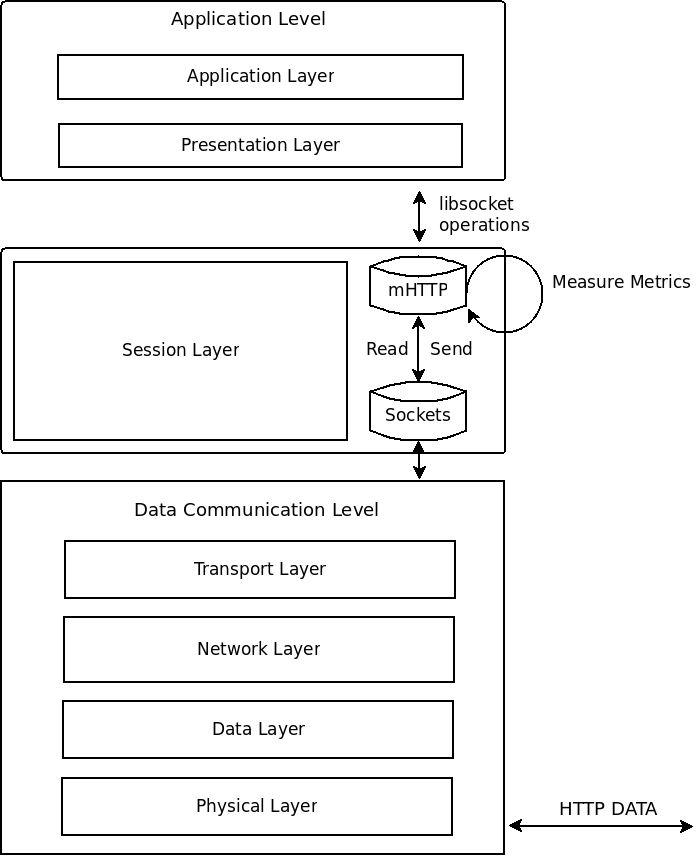
\includegraphics[width=\linewidth]{Figures/mhttp_layer_1}}
%        \end{center}
%        \end{minipage}
%~
        \begin{center}
			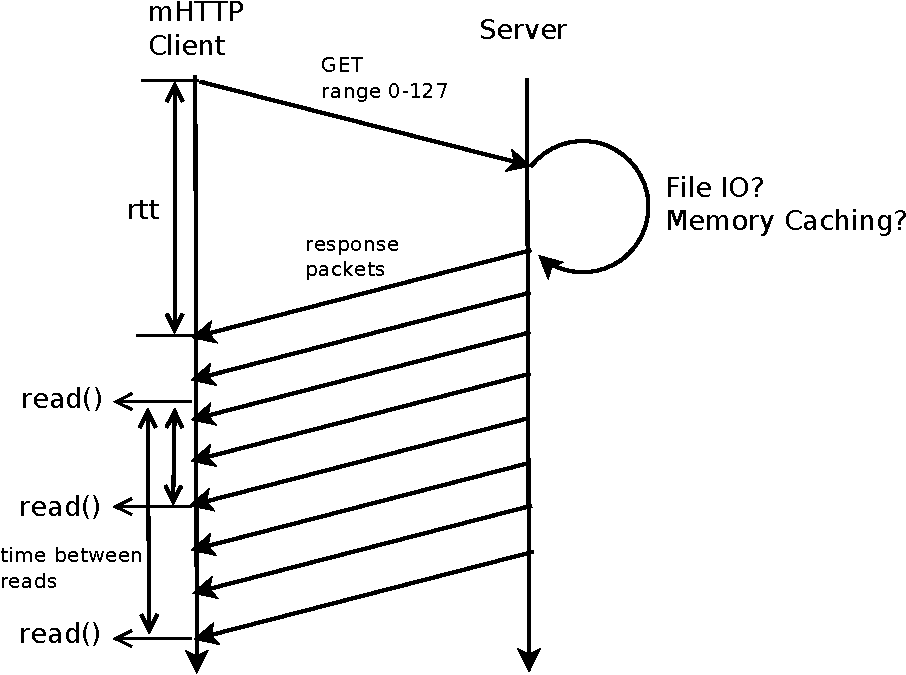
\includegraphics[width=0.7\linewidth]{Figures/scheduler-metrics}
        \end{center}
        \caption{Implications of Request/Response behavior for metrics estimation.}
		\label{fig:metrics}
  \vspace*{-0.3cm}
\end{figure*}

%This means that an event of receiving a byte has to go all the way up from the physical to the application layer which of course adds a certain amount of processing time and falsifies the real physically measured $rtl_i(n)$. 
TCP has a built in retransmission timer which decides when to resend a package after package loss. 
This timer bases its decision on an estimate of $\overline{rtl}_i$ which means that the TCP layer already has its own $\overline{rtl}_i$ estimate and in UNIX systems it is possible to access these values. 
The problem is that these calls are highly platform dependent. 
We try to avoid platform dependency and decide to measure the metrics ourselves inside the \mhttp~library. 
%Further measuring on the session/application layer would give us estimates that are valid on this layer and since our decisions are made for this layer, it is alright to use its estimates.
In order to estimate $rtl_i(n)$ we have to measure the time that goes by between the client sending the first byte of a request to the server and receiving the first byte of the response from the server as we can see in~\fref{fig:metrics}. 
This technique does not take into account the time necessary on the server to process the request until sending the first byte of the response. 
Further, depending on the server hardware and configuration this processing time differs from machine to machine. 
For instance a server that uses resource memory caching will, in most cases have a lower processing time than a server without caching, since reading a resource from disk comes with a huge overhead compared to reading from memory. 
This processing delay is usually comparatively smaller than the link propagation delay. 
%The good news here is that if the server is not overloaded and functioning normally, the processing time should be very small so neglecting it will not harm our estimate badly. 

We send a request to the server for each chunk. 
Directly before sending the request we save a timestamp. 
When the first read operation for the incoming response is performed we take another timestamp and calculate the difference between those two. 
That way we can fairly estimate the time difference between the first byte sent and the first byte received on our layer. 
It follows that during download time we would be able to obtain a new value for $rtl_{i}$ for each chunk request. 
This leads to the question on how to combine these estimates to obtain a more reliable one.
To estimate such a value from a set of samples, rather than simply using the basic mean we could learn from TCP. 
Since a normal mean would give too much importance to extreme values, we should rather consider using a weighed moving average like TCP does~\cite{RFC-6298}. 

On every socket read operation on $c_i$, we measure the current latency 
$rtl_{i}$  and estimate $\overline{rtl}_i$ using a weighed moving average:
$$\overline{rtl}_i = 0.8 \cdot \overline{rtl}_i + 0.2\cdot rtl_{i}.$$

Another issue is the throughput estimate $\overline{R}_i$. 
As we can see in~\fref{fig:metrics} (b) the throughput estimation could be performed by first saving the timestamp of the first socket read event and counting the number of bytes read since then. 
On every further socket read call we divide the total number of bytes since the beginning of the response by the time passed since the first read event. 
That way on every socket read operation (except for the very first one) we estimate single $R_{i}$ values on the \mhttp~layer. 
An important issue we have to consider is that the first read calls might return more bytes in a short amount of time than the following read calls. 
This is due to the fact that we do not measure directly the arrival of the packets on the link, but instead measure when the packets arrive in our \mhttp~layer. 
Until the first bytes are processed and ready for the \mhttp~layer to be read, a lot of bytes might already be buffered in the lower layers. 
This leads to a burst of data in the beginning once all the necessary structures are setup on all the other layers. 
To avoid that this burst falsifies our estimate, we simply neglect the first samples of the first read operations. 

We use the \term{harmonic mean} to estimate the throughput $\overline{R}_i$ on every socket read 
operation. Previous studies have shown that this provides a better throughput estimation
than a moving average estimate and mitigates the impact of large outliers due to 
network variation~\cite{CHEN14-MMA}. Given a series of bandwidth measurements $R_i(t)$, 
where $t=0,1,2,\cdots, n-1$, the \term{harmonic mean} is calculated as:
$$\overline{R}_i = \frac{n+1}{\frac{n}{\overline{R}_i} + \frac{1}{R_i(n+1)}}$$
